\section{Discussion}
This section provides the performance analyses of GenAU, highlighting challenges and insights that are often unexplored in prior studies.

\subsection{Local vs. Global Context Segmentation}
\begin{figure}[t]
  \centering
  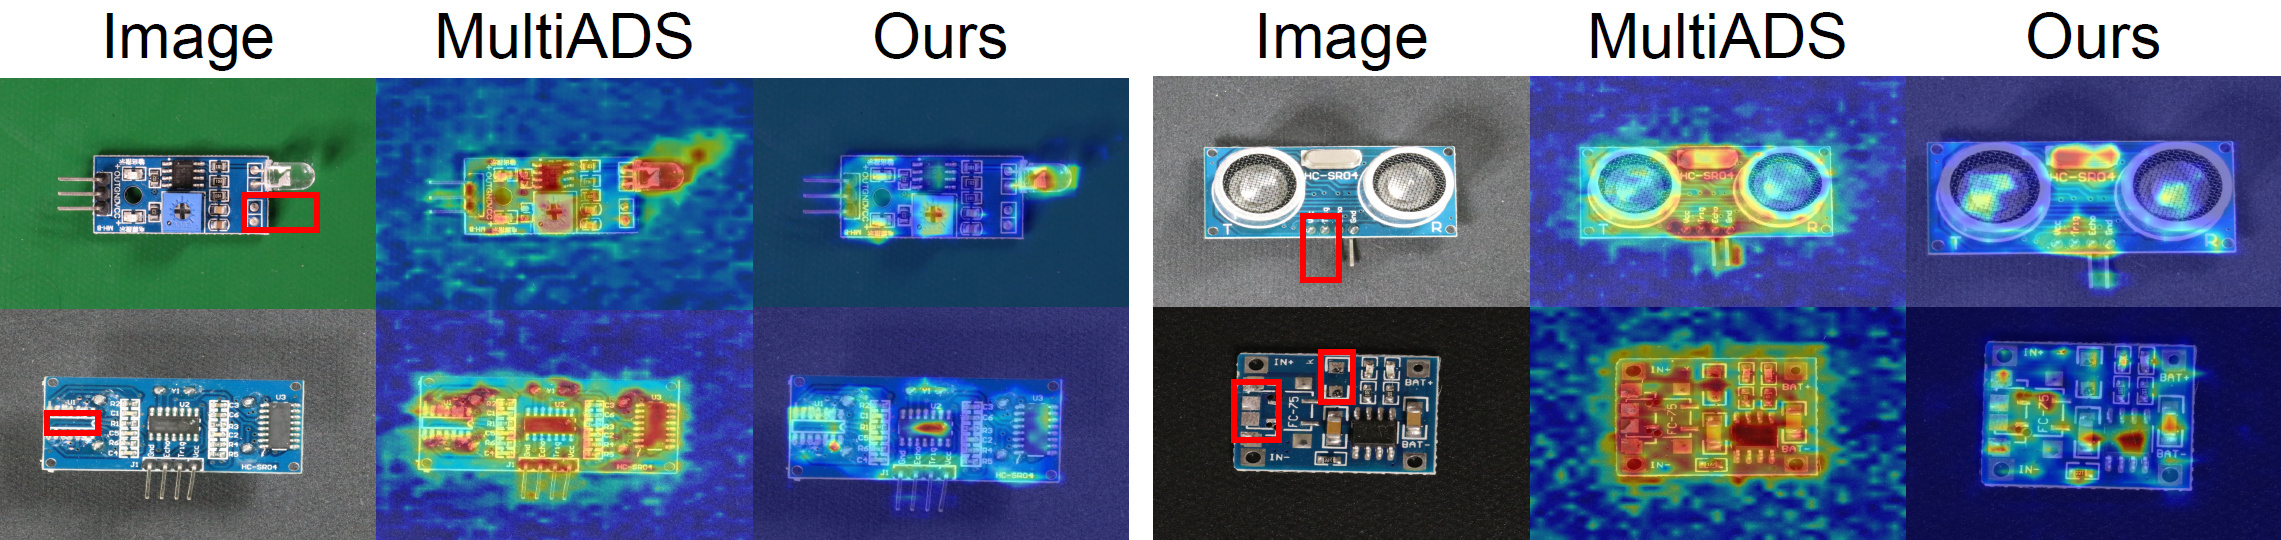
\includegraphics[width=1.0\columnwidth]{imgs/visa-missing.jpg}
  \caption{Anomaly segmentation on VisA for the \emph{missing} defect, a globally-defined anomaly, with MultiADS for comparison. Both methods yield low-confidence, incomplete maps.}
  \label{fig:visa-visual-bad}
\end{figure}
GenAU excels at visually salient anomalies (distinct texture or color deviations), where strong local cues align with the defect-token anchors. Segmentation degrades for globally-defined or logical anomalies (e.g., \textit{missing} or \textit{misplaced} components; Figure~\ref{fig:visa-visual-bad}), which look normal at the patch level and, in the zero-shot setting, give no prior on expected placement; few-shot or domain priors could help.

\subsection{Challenges in Defect-Type Classification}
Fine-grained classification exposes the limits of the VLM's pre-trained knowledge: the same label varies widely across objects (a \textit{missing cable} is a conspicuous void, a \textit{missing LED} blends in; cracks range from large openings to fine lines), so generalization is hard when training shows one instance of a defect. Logical defects further require reasoning about expected structure that the model cannot encode without domain knowledge; broader exposure to each defect would help.

\section{Conclusion}
We presented GenAU, an instruction-following VLM architecture for detection, localization, conditional defect-type recognition, and textual analysis. A single checkpoint, trained with reasoning conversations in half of its samples at an unchanged budget, provides competitive cross-dataset detection and localization and supports all four tasks; giving every sample a conversation doubles the budget and lowers detection and localization. Learned-query controls show a localization benefit on VisA, not universal superiority. Logical anomalies, fine-grained types, and verified causal diagnosis remain open challenges.





